% 本原稿用の条件マクロ
%章ごとにコンパイルできるようにするための設定.
%このマクロが定義されていない場合,チャプター内は個別のTEXソースとして扱われる.
\expandafter\ifx\csname MasterFile\endcsname\relax
\documentclass[a4j,twoside,12pt, dvipdfmx]{thesis} % 修論・卒論など (ページが右端にでる) 
\usepackage{amsmath, amssymb}
\usepackage{mysettings}
\usepackage{graphicx}
\usepackage{color}
\usepackage{comment}

\begin{document}

\addtocounter{chapter}{+2}

\setlength{\baselineskip}{1.95zw}
\setlength{\textheight}{30\baselineskip}
\mainmatter

\fi
% これより上は削除しちゃダメ
% 本原稿用の条件マクロここまで
%
%\newcommand{\argmax}{\mathop{\rm arg~max}\limits}
\renewcommand\thefootnote{\arabic{footnote})}
\def\vector#1{\mbox{\boldmath $#1$}}

\chapter{提案手法}\label{meth}
% ここに本文
本章では,研究手法について説明する.本研究は大きく分けて以下の 3 つに分類される.
\begin{enumerate}
  \item 文からのグラフ作成
  \item ノードの畳み込み
  \item グラフを表現する埋め込み生成
  \item グラフ間の類似度の評価
\end{enumerate}
\begin{figure}
  \centering
  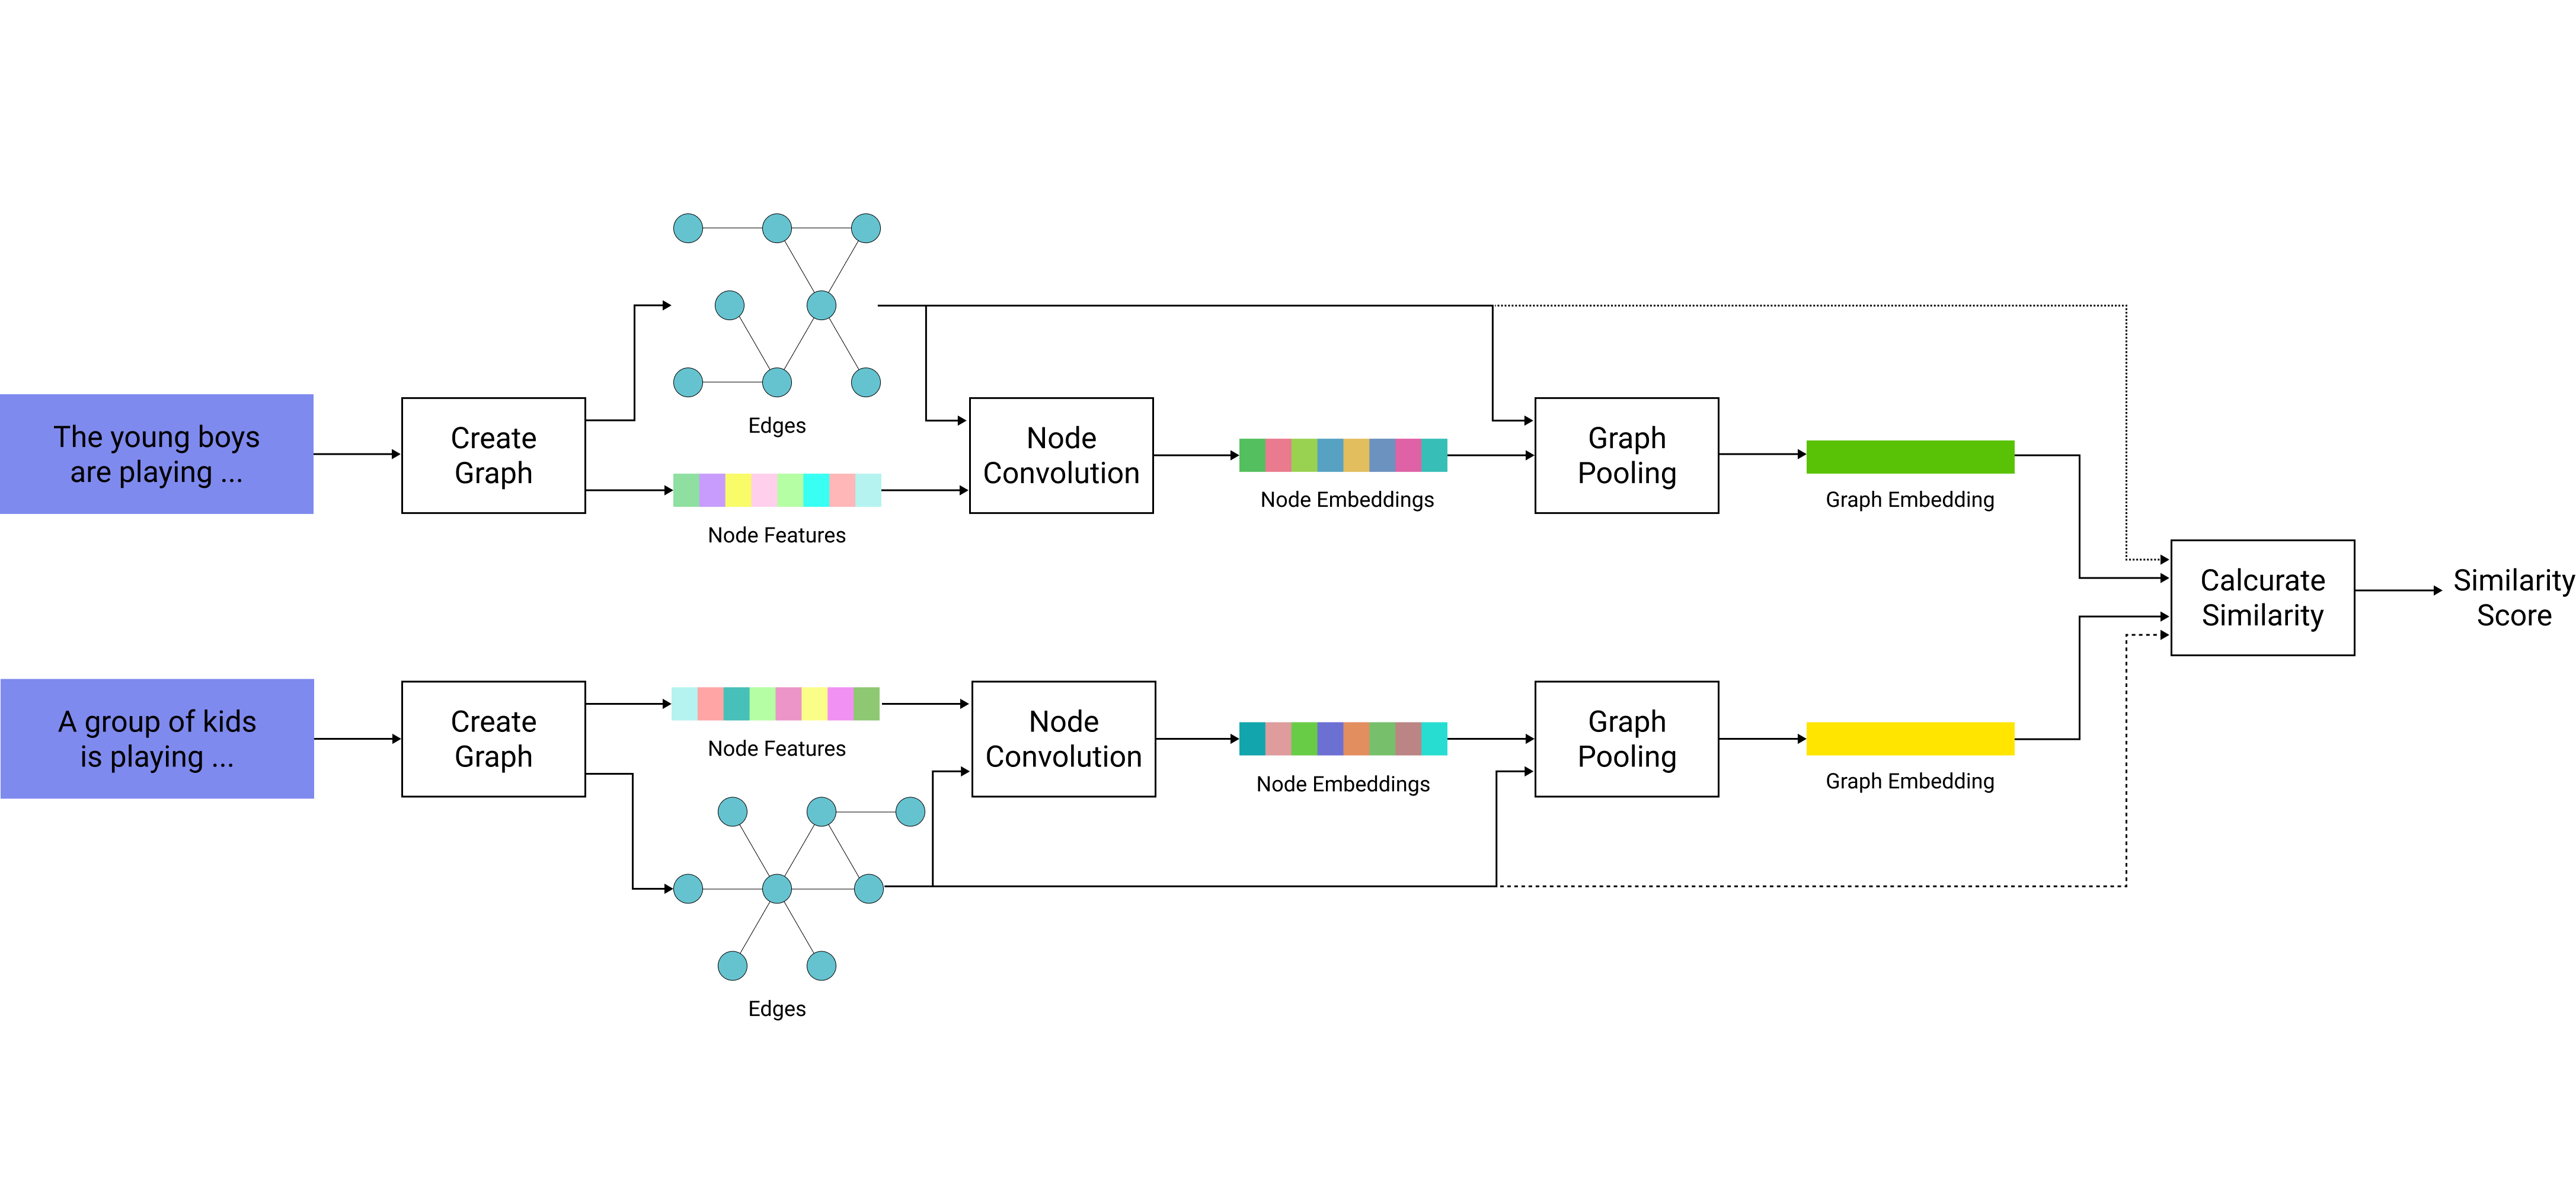
\includegraphics[width=\linewidth]
  {img/ModelFlow.jpg}
  \caption{モデルの概要}
  \label{ラベル名}
\end{figure}
\ref{meth:createGraph}節では文からのグラフ作成,\ref{meth:convNode}節ではノード畳込み \ref{meth:createEmbedding}節ではグラフを表現する埋め込み生成, \ref{meth:calculateSimilarity}節ではグラフ間の類似度計算について述べる.

\section{文からのグラフ作成}\label{meth:createGraph}
この節では,文からのグラフ生成方法について説明する.グラフの生成について,以下の2つを行う.
\begin{enumerate}
  \item ノード生成
  \item エッジ生成
\end{enumerate}
また, 本研究では以下の2通りのエッジ生成方法を元に, 2 種類のグラフを生成し実験した.
\begin{enumerate}
  \item 依存関係に基づくエッジ生成
  \item 依存関係と隣接関係に基づくエッジ生成
\end{enumerate}

\subsection{ノード生成}\label{meth:createNode}
文からのグラフの生成において,各ノードはそれぞれの単語とし,その単語のレンマの埋め込みを取得し,ノードの特徴量とする.

\subsection{エッジ生成}\label{meth:createEdge}
エッジの生成過程では2通りの方法を用いた.
\subsubsection{依存関係に基づくエッジ生成}
各エッジの生成には Universal Dependencies に基づく構文解析を行い,単語間に依存関係があれば双方向にエッジを作成し無向グラフを生成した.

\subsubsection{依存関係と隣接関係に基づくエッジ生成}
依存関係に基づくエッジ生成に加えて, 単語間に隣接関係があれば双方向エッジを作成した.

\section{ノードの畳込み}\label{meth:convNode}
この節では, ノードの畳込みについて説明する.

\subsection{Graph Convolutional Network (GCN)}
この手法では,Kipf ら\cite{kipf2017semi}と同様の GCN を用いる.
GCN の第$l$層における出力は以下の式で表される.
\begin{equation}H^{(l)}=f(\tilde{D}^{-\frac{1}{2}}\tilde{A}\tilde{D}^{-\frac{1}{2}}H^{(l-1)}W_{1}^{(l-1)})\end{equation}

\subsubsection{GraphSAGE}


\section{グラフを表現する埋め込み生成}\label{meth:createEmbedding}
この節では,グラフを表現する埋め込み生成方法について説明する.
この方法では, 前節の方法で得られたノードレベルの埋め込みを元にグラフを表現する埋め込みを生成する.
\subsection{Attention Module}
この方法は SimGNN\cite{bai2019simgnn}で用いられている Attention Module と同様のものである.
Attention Module から出力される, グラフを表現する埋め込み$h$は以下の式で表される.
\begin{equation}h = \sum_{n=1}^{N}\sigma(u_{n}^\mathsf{T}c)u_{n}= \sum_{n=1}^{N}\sigma(u_{n}^\mathsf{T} \tanh (\frac{1}{N}W_{2}\sum_{m=1}^{N}u_{m}))u_{n}\end{equation}
ここで, $u_{n}$ はノード$n$の埋め込み, $\sigma$ はシグモイド関数, $N$はノード数, $W_{2}$は学習可能な重みである.

\subsection{SAGPool}
\section{グラフ間の類似度計算}\label{meth:calculateSimilarity}
この節では, グラフ間の類似度計算について説明する.
この方法では, 前節の方法で得られたグラフを表現する埋め込みから類似度を計算する.

\subsection{Neural Tensor Network}
この方法は SimGNNで用いられている Neural Tensor Network と同様のものである.
2 つのグラフの埋め込み$h_{i}$, $h_{j}$を Neural Tensor Network に与えた出力は式\ref{eq:NTN}である.
\begin{equation} \label{eq:NTN} g(h_{i}, h_{j})=f(h_{i}^\mathsf{T}W_{3}^{[1:K]}h_{j} + V \begin{bmatrix} h_{i}\\h_{j} \end{bmatrix} + b)\end{equation}
を用いる.
ここで,$W_{3}^{[1:K]} \in R^{D \times D \times K}$は重み行列,$\begin{bmatrix} $ $ \end{bmatrix}$は結合操作,$V \in \mathbb{R}^{K\times2D}$は重みベクトル.
$b \in \mathbb{R}^{K}$はバイアスベクトル, $f(\cdot)$は$ReLU(\cdot) = \max (0, \cdot)$のような活性化関数である.得られた出力を 2 層の全結合層に与えることで, 最終的な類似度を得る.

\subsection{コサイン類似度}
2 つのグラフの埋め込み$h_{i}$, $h_{j}$のコサイン類似度は, 以下の式で表される.
\begin{equation} \label{eq:cos} \cos(h_{i}, h_{j}) = \dfrac{h_{i} \cdot h_{j}}{|h_{i} | | h_{j}|}\end{equation}

% 本原稿用の条件マクロ
% これ以降は削除しちゃダメ
\expandafter\ifx\csname MasterFile\endcsname\relax
\def\MasterFile{本原稿です}

% 参考文献
%% 本原稿用の条件マクロ
%章ごとにコンパイルできるようにするための設定.
%このマクロが定義されていない場合,チャプター内は個別のTEXソースとして扱われる.
\expandafter\ifx\csname MasterFile\endcsname\relax
\documentclass[a4j,12pt]{thesis} % 修論・卒論など (ページが右端にでる)   
\usepackage{mysettings}
\usepackage{url}

\begin{document}

\setlength{\baselineskip}{1.95zw}
\setlength{\textheight}{30\baselineskip}
\backmatter

\fi
% これより上は削除しちゃダメ
% 本原稿用の条件マクロここまで

%参考文献

\bibliographystyle{junsrt}
\bibliography{thesisB}

\clearpage


% 本原稿用の条件マクロ
% これ以降は削除しちゃダメ
\expandafter\ifx\csname MasterFile\endcsname\relax
\def\MasterFile{本原稿です}
\end{document}
\fi
% 本原稿用の条件マクロここまで


\bibliographystyle{sieicej}
\bibliography{thesisB}

\end{document}
\fi
% 本原稿用の条件マクロここまで
